\section{Edge Detection}
\label{sec:edge-detection}

Edge detection is a fundamental task in image processing and computer vision, aimed at identifying points in an image where the intensity changes sharply. These points typically correspond to object boundaries and other significant features within the image.

The gradient of an image is a vector that has both magnitude and direction. The magnitude indicates the strength of the edge, while the direction indicates the orientation of the edge (to be more precise, the shape of the object).

\subsection{Sobel Operator}
\label{subsec:sobel-operator}

The \emph{Sobel operator} is a widely used edge detection technique that employs two convolution kernels to estimate the gradient of the image intensity. One kernel is used to calculate the gradient in the x-direction, while the other is used to calculate the gradient in the y-direction.

\paragraph{Sobel Operator in the x-direction}
The convolution kernel for the \emph{Sobel} operator in the x-direction is defined as:
\begin{equation}
    G_x =
    \begin{bmatrix}
        -1 & 0 & 1 \\
        -2 & 0 & 2 \\
        -1 & 0 & 1
    \end{bmatrix}
    \label{eq:sobel_x}
\end{equation}

\paragraph{Sobel Operator in the y-direction}
The convolution kernel for the \emph{Sobel} operator in the y-direction is defined as:
\begin{equation}
    G_y =
    \begin{bmatrix}
        -1 & -2 & -1 \\
        0  & 0  & 0  \\
        1  & 2  & 1
    \end{bmatrix}
    \label{eq:sobel_y}
\end{equation}

\subsection{Magnitude and Direction of the Gradient}
\label{subsec:magnitude-and-direction}

The gradient magnitude and direction are essential for understanding the strength and orientation of edges in an image. These can be computed using the gradients in the x and y directions, \( G_x \) and \( G_y \), respectively.

\paragraph{Gradient Magnitude}
The magnitude of the gradient can be calculated using two different norms:

\begin{itemize}
    \item \textbf{L1 Norm:}
          \begin{equation}
              \text{Magnitude}_{L1} = |G_x| + |G_y|
              \label{eq:grad-magnitude-l1}
          \end{equation}
    \item \textbf{L2 Norm:}
          \begin{equation}
              \text{Magnitude}_{L2} = \sqrt{G_x^2 + G_y^2}
              \label{eq:grad-magnitude-l2}
          \end{equation}
\end{itemize}

\paragraph{Gradient Direction}
The direction of the gradient indicates the orientation of the edge and is computed as follows:
\begin{equation}
    \text{Direction} = \arctan\left(\frac{G_y}{G_x}\right)
    \label{eq:grad-direction}
\end{equation}

The gradient direction is typically measured in radians and can be converted to degrees if needed.

The result of applying the Sobel operator to an image is shown in \autoref{fig:sobel-gradient}.

\begin{figure}[ht]
    \centering
    \begin{subfigure}[b]{0.4\textwidth}
        \centering
        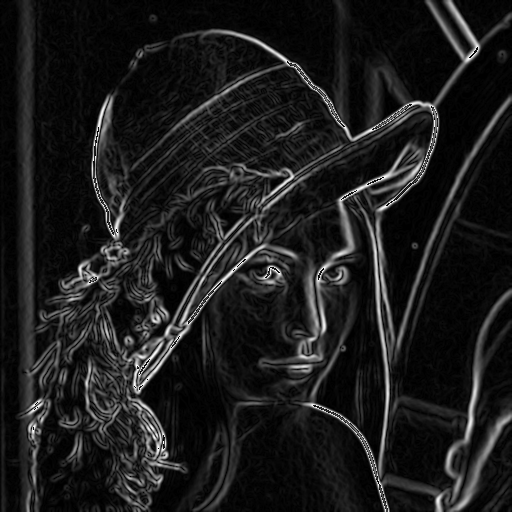
\includegraphics[width=0.9\textwidth]{lenna_4_gradient_magnitude.png}
        \caption{Gradient Magnitude}
        \label{fig:gradient-magnitude}
    \end{subfigure}
    \hfill
    \begin{subfigure}[b]{0.4\textwidth}
        \centering
        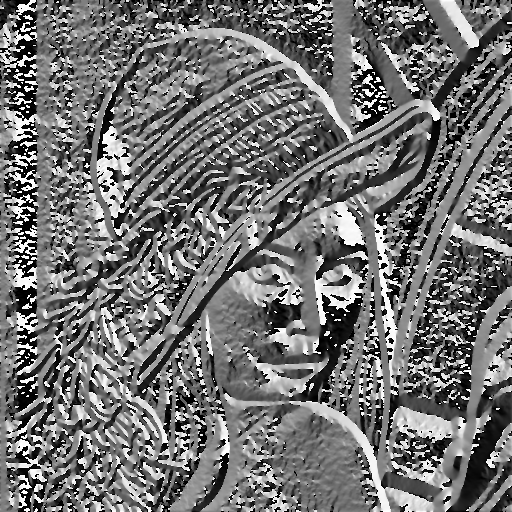
\includegraphics[width=0.9\textwidth]{lenna_5_gradient_direction.png}
        \caption{Gradient Direction}
        \label{fig:gradient-direction}
    \end{subfigure}
    \caption{Gradient Magnitude and Direction using Sobel Operator}
    \label{fig:sobel-gradient}
\end{figure}


It is important to note in \autoref{fig:gradient-direction} that the gradient direction can have both positive and negative values. Consequently, when visualizing the image, negative values are automatically truncated.